\documentclass[12pt,halfparskip]{scrartcl}

\usepackage{proposal}

\begin{document}

\pagestyle{plain}

\section*{Structural Analyser for Python – Project Proposal}
\vspace{-0.5cm}

\emph{by Reto Schüttel \& Robin Stocker, 12th February 2008}

\vspace{-0.3cm}

\subsection*{Introduction}

Planning and analysing a program's structure and internal dependencies is a common task when working on larger projects. Such analysis helps to meet the defined architectural design goals or to find structural flaws like cyclic dependencies. A clear architecture becomes more and more important as software grows.

The project's goal is to develop a structural analyser for programs written in the Python programming language. The analyser should be able to parse an application's source code and generate a graph representing its internal dependencies between methods, classes and modules. 

(1) The generated representation can be used for various further analysis. Headway Software developed a program structure analyser (Structure 101g) which takes such a dependency graph and visualises it. The data is exchanged between the analyser and Structure 101g using XML files.

(2) Of course the dependency representation can be used for other purposes as well.

\begin{figure}[h] \centering
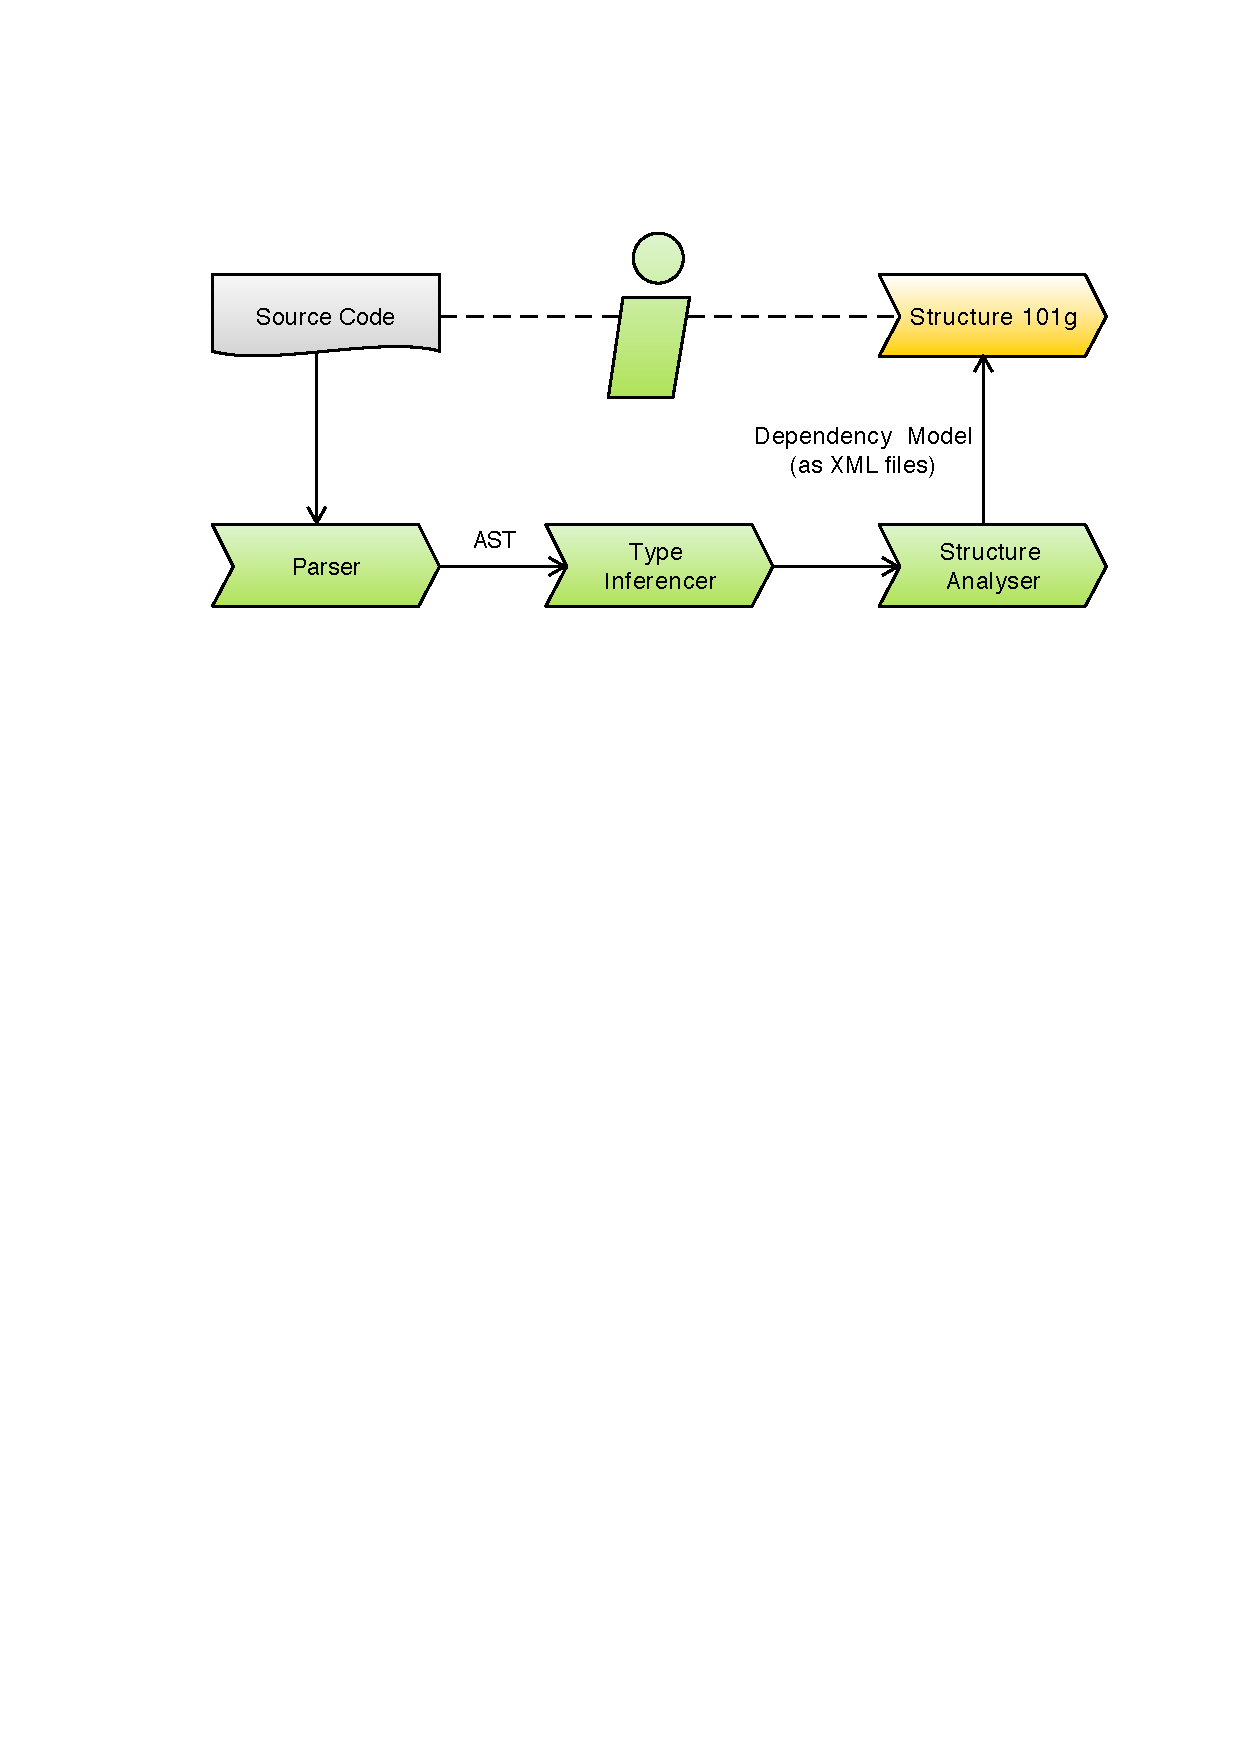
\includegraphics[width=0.75\textwidth]{big_picture}
\end{figure}


\subsection*{Analyser}

The analyser's main goal is to generate a graph which represents the internal structure of a program. First the source code has to be parsed and all the involved components such as modules, classes and methods have to be identified. The analyser then has to determine what variables, attributes and parameters are being used in these components and what types the variables have. This information can then be used to identify dependencies between different components. For example if method \id{b} gets called in method \id{a} the analyser has to identify a dependency between method \id{a} and method \id{b}. All these components and dependencies have to be incorporated into a graph which then can be used by \emph{Structure 101g} or other tools for further analysis or visualisation. 

\subsection*{Type Inference Engine}

Because types in a dynamic language are not known before the execution, a heuristic called type inference engine has to be used which tries to determine the types of variables in advance. In our previous term project, we developed such an engine to increase the accuracy of rename refactorings for Python. 

To use this engine in the project, the following improvements have to be made:

\begin{itemize}
	\item Add support for more language features like container types (lists, dicts, etc.)
	\item In case of type inference ambiguities, the user should be assisted with meaningful diagnostic messages
	\item Instead of focusing on a single variable, as in the rename refactoring, the engine has to analyse the whole project
\end{itemize}

\subsection*{Conceptual Questions}

For Java, structural analysis has turned out to be a valuable instrument, but for Python these techniques are not (yet) used often. The project should do some research on this topic and try to answer the following questions:

\begin{itemize}
	\item Is structural analysis also helpful for dynamic languages like Python?
	\item Are existing Python projects even suitable for structural analysis?
	\item \ldots or does fulfilling the needs of the analyser require extensive care during the development?
	\item What's the Python community's opinion about structural analysis?
\end{itemize}

\subsection*{Possible Challenges}

\begin{itemize}
	\item The type inference engine has to be able to detect implicit abstraction. Due to the nature of type inference, the engine only finds \emph{concrete} types (like \id{car} or \id{plane}) for variables, but never \emph {abstract} types (like \id{vehicle}). The implicitly used base class has to be guessed using the information provided by the context. For example: if a method processes planes and cars, but only the method \id{repair} of the common base class \id{vehicle} is being called, the engine should automatically guess that the developer implicitly intended to handle the passed parameter as object of the base class \id{vehicle}. In Java this intention is explicitly declared.
	\item How does the type inference algorithm scale to large projects? What is the impact of using XML as a data exchange format?
\end{itemize}


\end{document}
